% STATS 401 - Individual Project: one-slide summary
% Compile with pdfLaTeX from this folder. Images:
%   ZkXLXsV9ZJ-1350.png        the original figure (the repo's .webp converted
%                              to PNG, because LaTeX cannot read WebP)
%   redesign.png               screenshot of the redesign, shown in full
% The original figure is 147 rows long, so its \includegraphics uses
% trim=<left> <bottom> <right> <top> with clip to show the top rows.
\documentclass[aspectratio=169,10pt]{beamer}
\usepackage[T1]{fontenc}

\usetheme{default}
\setbeamertemplate{navigation symbols}{}
\setbeamersize{text margin left=5mm,text margin right=5mm}

\definecolor{ink}{HTML}{0B0B0B}
\definecolor{muted}{HTML}{52514E}
\definecolor{accent}{HTML}{184F95}
\definecolor{strength}{HTML}{006300}
\definecolor{weakness}{HTML}{B5322F}

\setbeamercolor{normal text}{fg=ink}
\setbeamercolor{frametitle}{fg=ink}
\setbeamerfont{frametitle}{size=\large,series=\bfseries}
\setbeamerfont{framesubtitle}{size=\footnotesize}
\setbeamercolor{framesubtitle}{fg=muted}

\setbeamertemplate{footline}{%
  \hspace{5mm}{\tiny\color{muted}%
  Live page: \texttt{blackcatyu.github.io/stats401-individual-project}%
  \hfill
  Data: World Happiness Report 2026, ``Data for Figure 2.1''; regions: World Bank}%
  \hspace{5mm}\vspace{2mm}}

% Column heading, and the small tags that tie each fix to a weakness.
\newcommand{\coltitle}[1]{{\small\bfseries\color{accent}#1}\par\vspace{1.2mm}}
\newcommand{\wtag}[1]{{\setlength{\fboxsep}{1.2pt}\colorbox{weakness}{\textcolor{white}{\tiny\bfseries W#1}}}}
\newcommand{\plus}{\textcolor{strength}{\bfseries +}}
% \point[label width]{label}{text}: a hanging-indent item.
\newcommand{\point}[3][5.5mm]{\noindent\hangindent=#1\hangafter=1\makebox[#1][l]{#2}#3\par\vspace{1mm}}

\begin{document}

\begin{frame}[t]
\frametitle{Redesigning the World Happiness Report ranking chart}
\framesubtitle{STATS 401 Individual Project: Visualization Critique and Redesign}

\vspace{-2.5mm}
\begin{columns}[T,onlytextwidth]

  % 1. Original ---------------------------------------------------------------
  \begin{column}{0.22\textwidth}
    \coltitle{1. Original}
    % 1350 x 4190 px in full; the trim keeps the title and the top 56 rows.
    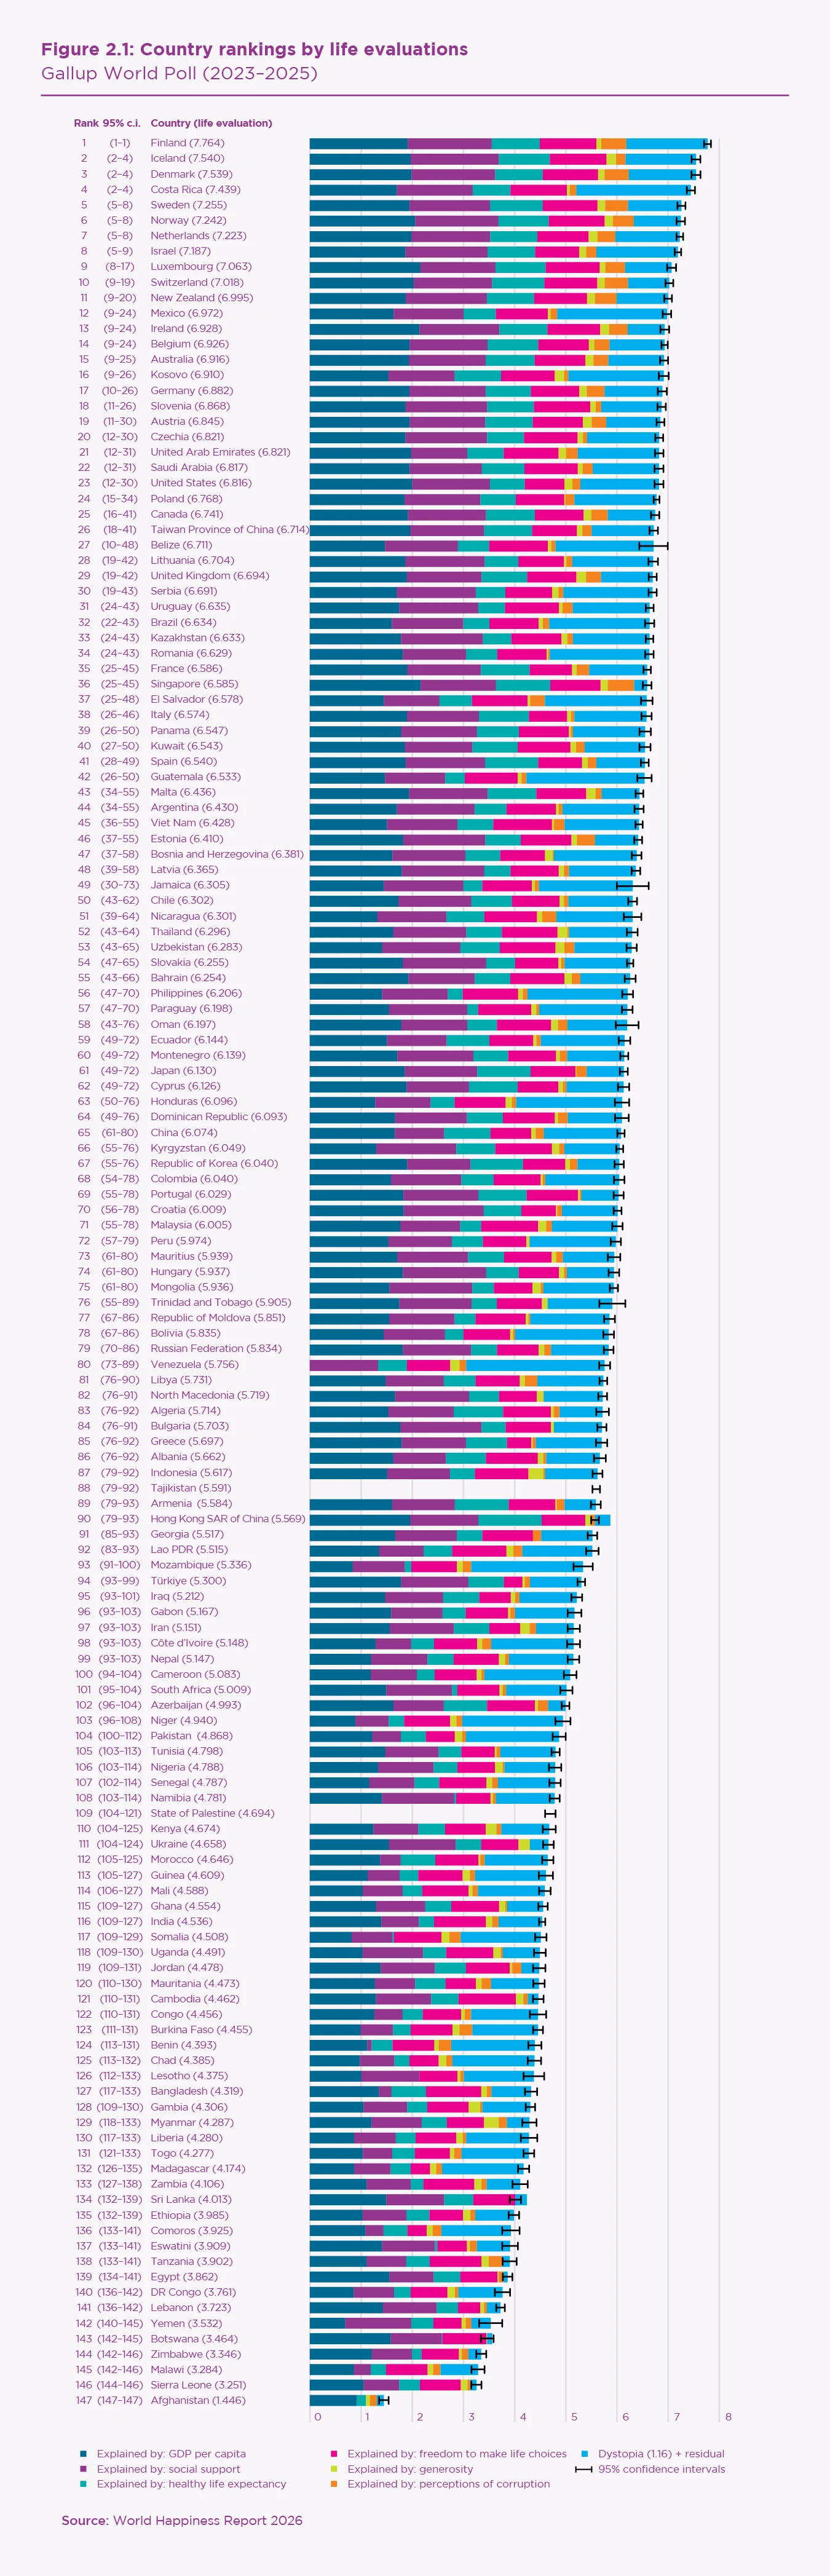
\includegraphics[width=\linewidth,trim=60 2562 60 40,clip]{ZkXLXsV9ZJ-1350.png}\par\vspace{1mm}
    {\scriptsize\color{muted}
      \emph{World Happiness Report 2026}, Fig.~2.1 (top 56 of 147 rows).
      Bar length = mean life evaluation (0--10); seven segments = six
      explanatory factors + ``Dystopia + residual''.\par}
  \end{column}

  % 2. Critique ---------------------------------------------------------------
  \begin{column}{0.33\textwidth}
    \coltitle{2. Critique}
    \footnotesize
    {\bfseries Strengths}\par\vspace{0.8mm}
    \point{\plus}{Sorted bars on a common baseline: totals compare
      accurately (Cleveland \& McGill, 1984).}
    \point{\plus}{Uncertainty is shown: 95\% intervals for scores and ranks.}

    \vspace{0.8mm}
    {\bfseries Weaknesses}\par\vspace{0.8mm}
    \point{\wtag{1}}{Stacking implies the six factors add up to the score;
      the ranking actually uses survey answers only.}
    \point{\wtag{2}}{Only the first segment has a common baseline, so
      factors cannot be compared across countries.}
    \point{\wtag{3}}{147 ranked rows overstate tiny gaps (neighbors differ
      by about 0.02; intervals are about 0.22 wide) and hide regions.}
  \end{column}

  % 3. Redesign ---------------------------------------------------------------
  \begin{column}{0.42\textwidth}
    \coltitle{3. Redesign (D3.js, three linked views)}
    {\centering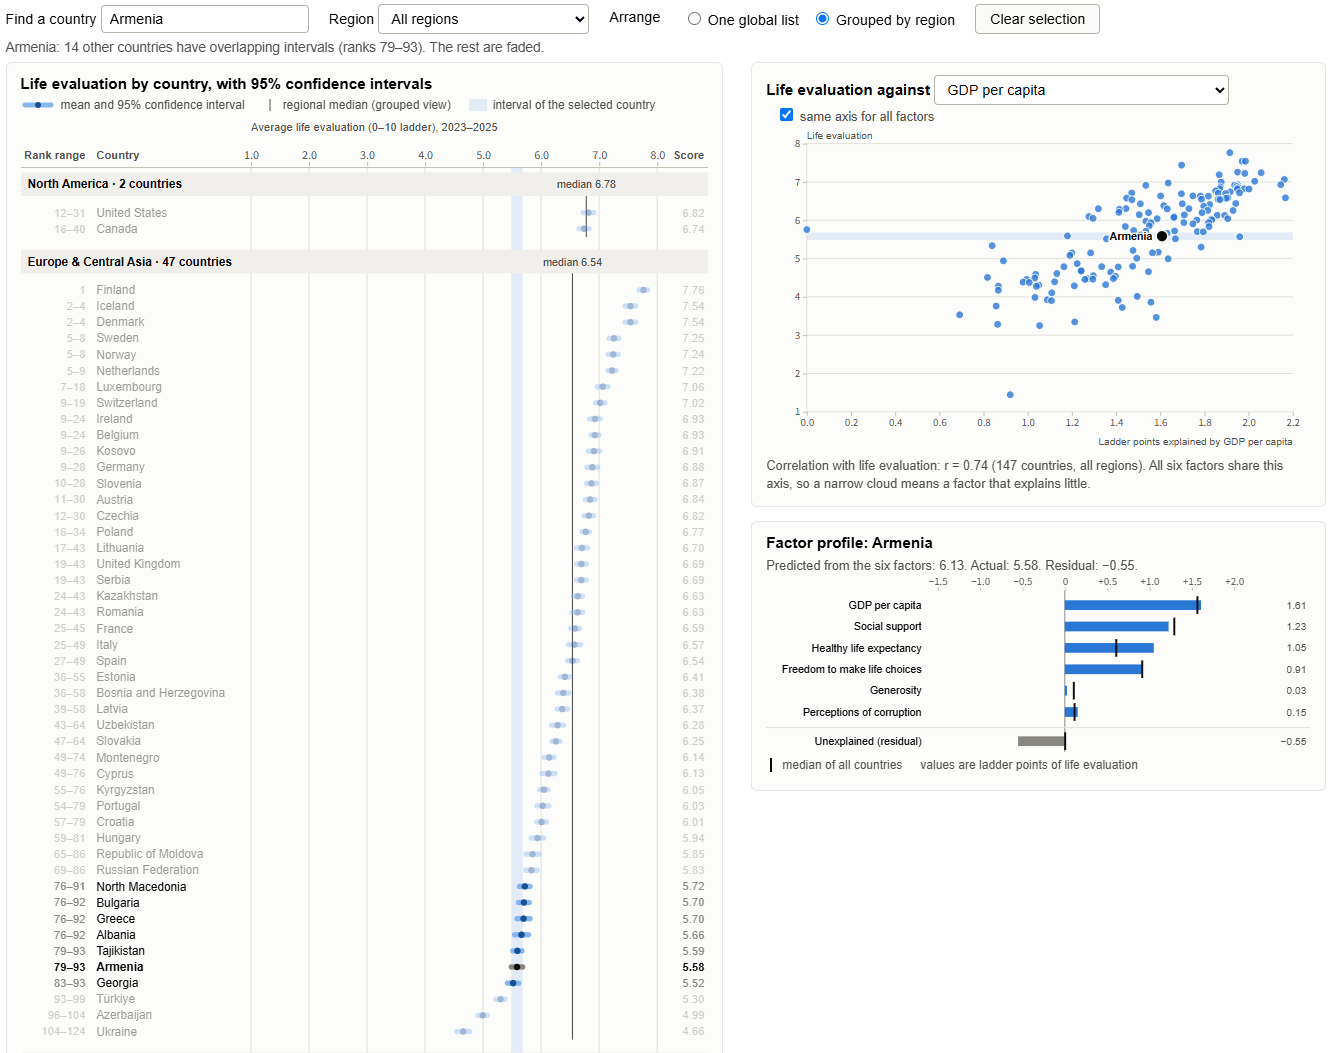
\includegraphics[height=36mm]{redesign.png}\par}\vspace{1.2mm}
    \footnotesize
    \point[10mm]{\wtag{3}}{Dots with 95\% intervals and rank ranges; selecting
      a country (here Armenia) fades clearly different ones.}
    \point[10mm]{\wtag{1}\,\wtag{2}}{One factor per axis against the score, plus
      a common-baseline profile; residual shown on its own.}
    \point[10mm]{\wtag{3}}{Grouped by region with median lines; filter and
      search; one hue instead of seven.}
  \end{column}

\end{columns}
\end{frame}

\end{document}
